\subsection{Linear Stability in One Dimension}
Consider a nearby orbit $x_n=\tilde{x}+\xi_n$ for a fixed point $\tilde{x}$
\begin{equation}
	\xi_{n+1}+\tilde{x}=f(x_n)\approx f(\tilde{x})+f^\prime(\tilde{x})\ \xi_n+\frac{1}{2!}f^{\prime\prime}(\tilde{x})\xi_n^2+\cdots
\end{equation}
$f(\tilde{x})=\tilde{x}$ as it is a fixed point.
$|\xi_n|$ is small as we assume to be in the vicinity of $\tilde{x}$, and therefore $\xi_n^2$ is tiny and can be neglected.
with \emph{eigenvalue} or {\textbf{multiplier}} $\lambda=f^\prime(\tilde{x})$
\begin{equation}
	\xi_{n+1}=f^\prime(\tilde{x})\ \xi_n=\lambda\ \xi_n\quad\rightarrow\quad\xi_n=\lambda^n\xi_0
\end{equation}
If $|\lambda|<1$, then fixed point $\tilde{x}$ is \textbf{linearly stable}.
For positive values of $\lambda$, $\xi_i=0$ is approached \emph{monotonically}, for a negative $\lambda$ the values of $\xi_i$ \emph{alternate} between positive and negative after each iteration step.
Conversely, if $|\lambda|>1$ then the fixed point is {\textbf{unstable}}.
\subsection{Graphical Iteration (Cobwebs)}
The general method for determining the itinerary of a seed $x_0$ for a function $f(x)$ is as follows
\begin{itemize}
	\item Start with the seed $x_0$ on the $x$-axis.
	\item Move up to the function $f(x)$.
	\item Move horizontally (left or right) to the $y=x$ line.
	\item Move vertically (up or down) to the function $f(x)$
	\item Repeat above two steps again and again.
\end{itemize}
Consider the \textbf{Tent Map} $T:[0,1]\rightarrow[0,1]$ defined by
\begin{equation}
	T(x)=
	\begin{cases}
		\mu x&0\leq x<\frac{1}{2}\\
		\mu(1-x)&\frac{1}{2}\leq x\leq1
	\end{cases}
\end{equation}
\begin{figure}[h!]
	\centering
	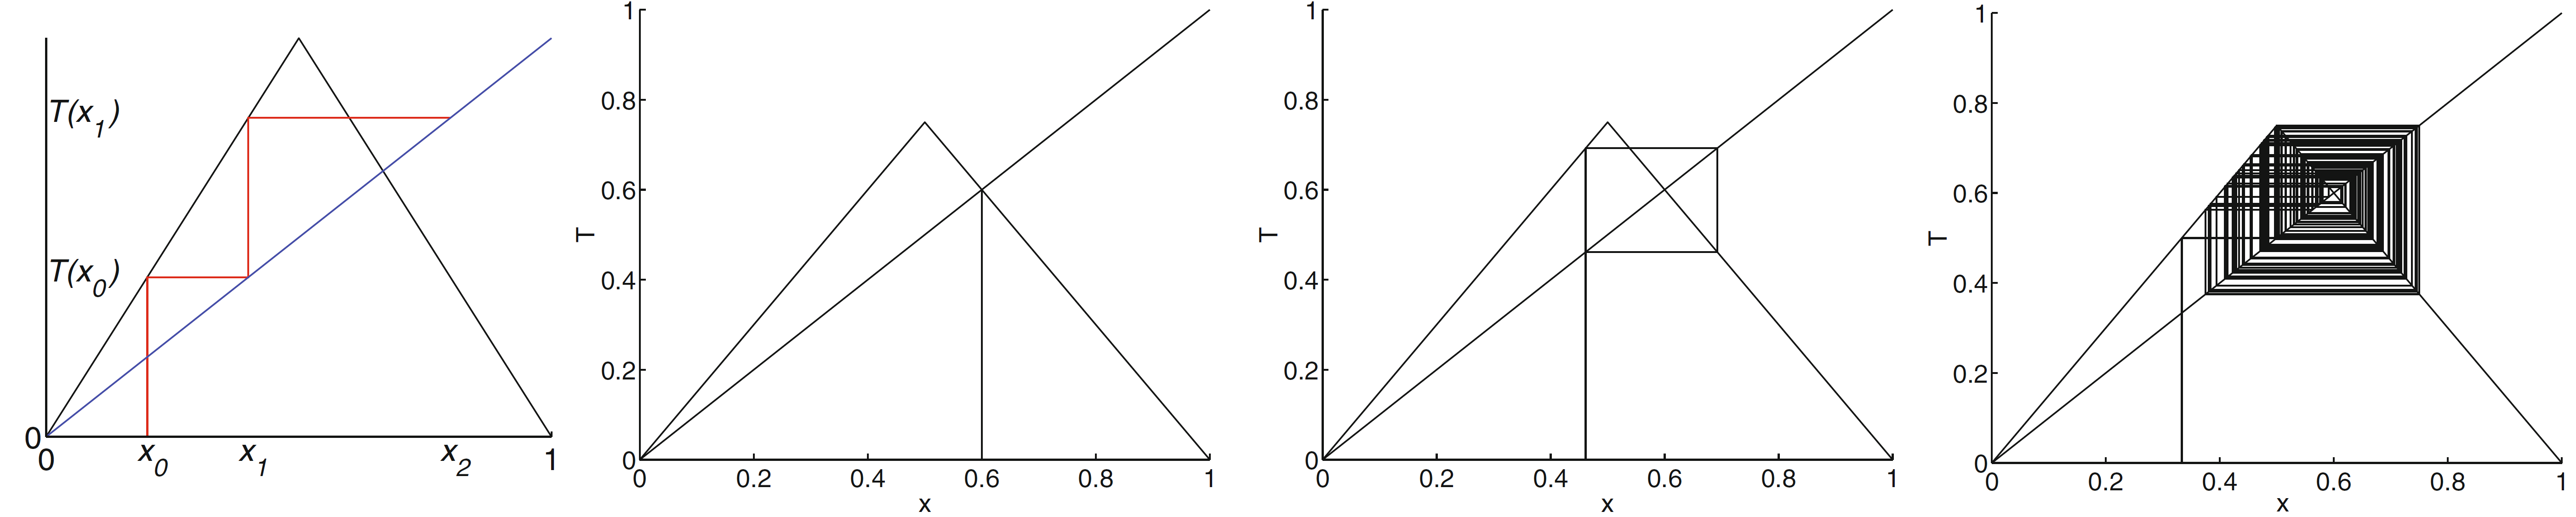
\includegraphics[width=0.83\linewidth]{cwd.png}
	\caption{a) A possible graphical iteration when n =2.\\Graphical iterations when $\mu=\frac{3}{2}$: b) $x_0=\frac{3}{5}$ c) $x_0=\frac{6}{13}$ d) $x_0=\frac{1}{3}$, for 200 iterations.}
	\label{fig:cwd}
\end{figure}